\section{Arsitektur Sistem}
Arsitektur sistem yang akan dikembangkan ditunjukkan dalam gambar \ref{fig:arsitektur_sistem} dimana antara \emph{client} dengan server merupakan dua bagian yang terpisah. Komunikasi antara \emph{client} dengan server dilakukan secara asinkron. 

Arsitektur RESTful dipilih dengan tujuan untuk penyederhanaan proses komunikasi antara \emph{client} dengan server serta untuk memudahkan pengembangan \emph{client} berbasis multi-platform. Server menerima \emph{request} pertanyaan dalam format \emph{plain text} atau objek JSON, kemudian respon diberikan dalam format ojek json.

\begin{figure}[ht]
    \centering
    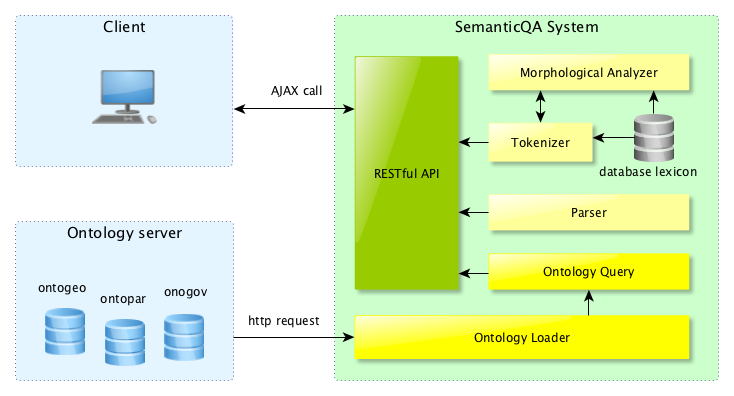
\includegraphics[width=1\textwidth]{arsitektur_sistem}
    \caption{Arsitektur sistem yang akan dikembangkan}
    \label{fig:arsitektur_sistem}
\end{figure}

Masing-masing ontologi diletakkan di lokasi yang berbeda dan dapat diakses secara terpisah melalui protokol HTTP.